\documentclass[12pt,a4paper]{article} 

\usepackage{fn2kursstyle}
\usepackage[russian]{babel}
\usepackage[T2A]{fontenc} 
\usepackage[utf8]{inputenc} 
\usepackage{geometry}
\usepackage{graphicx}
\usepackage{mathtools}
\usepackage{tikz}
\usepackage{pdfpages}
\usepackage{booktabs}
\usepackage{multirow,array}
\usepackage{siunitx}
\usepackage{amsmath}
\usepackage[hidelinks]{hyperref}

\counterwithout{equation}{section}
\counterwithout{figure}{section}
\graphicspath{{../pic/}}
\frenchspacing 

\newcolumntype{C}[1]{>{\centering\arraybackslash}p{#1}}

\newcommand{\picref}[1]{рис. \ref{#1}}
\newcommand{\tabref}[1]{таблица \ref{#1}}
\newcommand{\half}{\frac{1}{2}}
\newcommand{\dhalf}{\dfrac{1}{2}}
\newcommand{\dpartial}[2]{\dfrac{ \partial #1 }{ \partial #2 }}
\newcommand*{\Scale}[2][4]{\scalebox{#1}{$#2$}}

\title{КУСОЧНО-ПАРАБОЛИЧЕСКИЙ МЕТОД НА ЛОКАЛЬНОМ ШАБЛОНЕ ДЛЯ РЕШЕНИЯ ЗАДАЧ ГАЗОВОЙ ДИНАМИКИ}
\group{ФН2-72Б}
\author{А.\,И.~Токарев}
\supervisor{В.\,В.~Лукин}
\date{2022}

\begin{document}
    \maketitle
    \tableofcontents
    \pagebreak

    \section-{Введение}

    В рамках предыдущей работы проводилось сравнение кусочно-параболического метода (с англ. Piecewise-Parabolic Method, PPM) и его модификации – кусочно-параболического метода на локальном шаблоне (PPML). Его отличительными особенностями являются сохранение инвариантов Римана, уменьшение осцилляций на разрывных решениях, простота распараллеливания алгоритма. 

    Целью данной курсовой работы является решение задач газовой динамики с применением метода PPML. В общем случае такая система имеет $3$ характеристики, вдоль которых сохраняются решения. В задаче на одномерное уравнение переноса характеристика в каждой точке всего одна, каждая из них параллельна всем остальным. Однако в случае с газовой динамикой, характеристики, выпущенные из 2 разных точек, могут пересечься. В таком случае образуется либо контактный разрыв, либо ударная волна. Таким образом, нужно будет решать задачу Римана на границах каждой разностной ячейки.

    Кроме того, система уравнений газовой динамики нелинейная. Для применения метода PPML необходимо будет определять базис собственных векторов на каждом отрезке. Этот подход дает возможность линеаризовать систему в окрестности каждой такой ячейки.
    
    Тестирование метода PPML будет проводиться на одномерных и двумерных задачах газовой динамики.

    \newpage
    
    \section{Постановка задачи}

    \subsection{Одномерный случай} 

    Запишем систему газовой динамики:
    \begin{equation}
        \label{system:1d}
        \dfrac{\partial \bold u}{\partial t} + \dfrac{\partial \bold F}{\partial x} = 0,
    \end{equation}
    \noindent где 
    \begin{gather*}
        \bold u = \bigl(\rho, \rho u, e \bigr)^T, \quad \bold F = \bigl(\rho u, \rho u^2 + P, (e + P) u \bigr)^T, \\[0.7em]
        e = \rho \varepsilon + \dfrac{\rho u^2}{2}
    \end{gather*}

    Систему (\refeq{system:1d}) нужно дополнить уравнением состояния идеального газа:
    \begin{equation}
        \label{eq:gas}
        P = (\gamma - 1) \rho \varepsilon, \quad \gamma = \Biggl\{ \dfrac{5}{3}, \dfrac{7}{5} \Biggr\}
    \end{equation}

    Для более простого вывода собственных числел и векторов системы (\refeq{system:1d}), перейдем к неконсервативным (физическим) переменным:
    \begin{equation} 
        \label{var1d:phys}
        \bold v = (\rho, u, P)^T,
    \end{equation}

    \begin{enumerate}
        \item $ \dfrac{\partial \rho}{\partial t} + \dfrac{\partial \rho u}{\partial x} = 0 \Rightarrow \dfrac{\partial \rho}{\partial t} + u \dfrac{\partial \rho}{\partial x} + \rho \dpartial{u}{x} = 0;$ \\[0.5em]
        
        \item $ \dpartial{\rho u}{t} + \dpartial{[\rho u^2 + P]}{x} = 0 \Rightarrow $ \\[2mm]
        $ \dpartial{\rho u}{t} = u \dpartial{\rho}{t} + \rho \dpartial{u}{t} \overset{(1)}{=} \rho \dpartial{u}{t} - u \dpartial{\rho u}{x} $, \\[3mm]
        $ \dpartial{[\rho u^2 + P]}{x} = \dpartial{[\rho u \cdot u + P]}{x} = u \dpartial{\rho u}{x} + \rho u \dpartial{u}{x} + \dpartial{P}{x} $ \\[3mm]
        $ \quad \Rightarrow \dpartial{u}{t} + u \dpartial{u}{x} + \dfrac{1}{\rho} \dpartial{P}{x}= 0; $ \\[0.2em]

        \item $ \dpartial{e}{t} + \dpartial{[(e+ P) u]}{x} = 0 \Rightarrow \dfrac{1}{\gamma - 1} \dpartial{P}{t} + \dfrac{1}{2} \dpartial{\rho u^2}{t} + \dpartial{\Bigl[ \Bigl( \tfrac{\gamma}{\gamma - 1} P + \tfrac{1}{2} \rho u^2 \Bigr) u \Bigr]}{x} = 0 \Rightarrow $ \\[2mm]
        $\dfrac{1}{2} \dpartial{\rho u^2}{t} = \dhalf u \dpartial{\rho u}{t} + \dhalf \rho u \dpartial{u}{t} \overset{(1, 2)}{=} - \rho u^2 \dpartial{u}{x} - \dhalf u^2 \dpartial{\rho u}{x} - u \dpartial{P}{x} $ \\[3mm]
        $ \dpartial{\Bigl[ \Bigl( \tfrac{\gamma}{\gamma - 1} P + \tfrac{1}{2} \rho u^2 \Bigr) u \Bigr]}{x} = \rho u^2 \dpartial{u}{x} + \dfrac{\gamma}{\gamma - 1} P \dpartial{u}{x} + \dfrac{\gamma}{\gamma - 1} u \dpartial{P}{x} + \dhalf u^2 \dpartial{\rho u}{x}$ \\[2mm]
        $ \Rightarrow \dpartial{P}{t} + \gamma P \dpartial{u}{x} + u \dpartial{P}{x} = 0, $ \\
      \end{enumerate}  

      \noindent откуда получается матрица, собственные числа и соответующие им векторы которой являются собственными значениями и векторами системы (\refeq{system:1d})
      \begin{equation}
        \label{eigen1d}
        \begin{array}{c}
                A = \begin{pmatrix}
                    u & \rho & 0 \\
                    0 & u & \dfrac{1}{\rho} \\
                    0 & \gamma P & u
                \end{pmatrix}, \quad
                \Lambda = (
                    u - c,\, u,\, u + c
                )^T, \\
                R = \begin{pmatrix}
                    1 & 1 & 1 \\[2mm]
                    -\dfrac{c}{\rho} & 0 & \dfrac{c}{\rho} \\[4mm]
                    c^2 & 0 & c^2
                \end{pmatrix}, \quad 
                L = \begin{pmatrix}
                    0 & -\dfrac{\rho}{2c} & \dfrac{1}{2c^2} \\[3mm]
                    1 & 0 & -\dfrac{1}{c^2} \\[3mm]
                    0 & \dfrac{\rho}{2c} & \dfrac{1}{2 c^2}
                \end{pmatrix}, \quad 
            \end{array}
    \end{equation}

        \subsection{Двумерный случай}

        Система газовой динамики в случае движения не только по оси $Ox$, но и $Oy \colon$
        \begin{equation}
            \label{system:2d}
            \dpartial{\bold u}{t} + \dpartial{\bold F}{x} + \dpartial{\bold G}{y} = 0,
        \end{equation}
        \noindent где 
        \begin{gather*}
            \bold u = (\rho, \rho u, \rho v, e)^T, \quad \bold F = (\rho u, \rho u^2 + P, \rho u v, (e + p) u)^T, \\
            \bold G = (\rho v, \rho u v, \rho v^2 + P, (e + P) v)^T, \quad e = \rho \varepsilon + \rho \dfrac{u^2 + v^2}{2}.
        \end{gather*}

        Уравнение состояния (\refeq{eq:gas}) актуально и для системы (\refeq{system:2d}), физические переменные представим в виде вектора:
        \begin{equation}
            \label{var2d:phys}
            \bold v = (\rho, u, v, P)^T.
        \end{equation}

        \pagebreak

        Выведем собственные числа и собственные векторы (\refeq{system:2d}):

        \begin{enumerate}
            \item $ \dpartial{\rho}{t} + \dpartial{\rho u}{x} + \dpartial{\rho v}{t} = 0 \Rightarrow \dpartial{\rho}{t} + u \dpartial{\rho}{x} + \rho \dpartial{u}{x} + v \dpartial{\rho}{y} + \rho \dpartial{v}{y} = 0; $ \\[0.7em]
            
            \item $ \dpartial{\rho u}{t} + \dpartial{[\rho u^2 + P]}{x} + \dpartial{\rho u v}{y} = 0 \Rightarrow $ \\[3mm]
            $ \dpartial{\rho u}{t} \overset{(1)}{=} \rho \dpartial{u}{t} - u \dpartial{\rho u}{x} - u \dpartial{\rho v}{y} $ \\[3mm]
            $ \Rightarrow \dpartial{u}{t} + u \dpartial{u}{x} + \dfrac{1}{\rho} \dpartial{P}{x} = 0; $ \\[0.7em]

            \item $ \dpartial{\rho v}{t} + \dpartial{ [\rho u v]}{x} + \dpartial{[\rho v^2 + P]}{y} \Rightarrow $ \\[3mm]
            $ \dpartial{\rho v}{t} = \rho \dpartial{v}{t} + v \dpartial{\rho}{t} = \rho \dpartial{v}{t} - v \dpartial{\rho u}{x} - v \dpartial{\rho v}{y} $ \\[3mm]
            $ \Rightarrow \dpartial{v}{t} + v \dpartial{v}{y} + \dfrac{1}{\rho} \dpartial{P}{y} = 0; $ \\[0.7em]

            \item $ \dpartial{e}{t} + \dpartial{[(e + P) u]}{x} + \dpartial{[(e + P) v]}{y} = 0, \quad e = \dfrac{P}{\gamma - 1} + \rho \dfrac{u^2 + v^2}{2} \Rightarrow $ \\[3mm]
            \[
                \begin{split}
                    \Rightarrow \dfrac{1}{\gamma - 1} \dpartial{P}{t} + \dhalf \dpartial{[\rho u^2]}{t} + \dhalf \dpartial{[\rho v^2]}{t} &+ \dpartial{\Bigl[ \Bigl( \dfrac{\gamma}{\gamma - 1} P + \rho \dfrac{u^2 + v^2}{2} \Bigr) u \Bigr]}{x} + \\
                    & + \dpartial{\Bigl[ \Bigl( \dfrac{\gamma}{\gamma - 1} P + \rho \dfrac{u^2 + v^2}{2} \Bigr) v \Bigr]}{y} = 0
                \end{split}  
            \]

            \[
                \hspace*{-1.75cm} \begin{split}
                    \dhalf \dpartial{\rho u \cdot u}{t} = u \dpartial{\rho u}{t} + \rho u \dpartial{u}{t} &\overset{(1)}{=} \rho u \dpartial{u}{t} - \dhalf u^2 \dpartial{\rho u}{x} - \dhalf u^2 \dpartial{\rho v}{y} \overset{(2)}{=} \\[3mm]
                    &= \rho u^2 \dpartial{u}{x} - u \dpartial{P}{x} - \dhalf u^2 \dpartial{\rho u}{x} - \dhalf u^ 2\dpartial{\rho v}{y}
                \end{split}  
            \]

            $ \dhalf \dpartial{\rho v^2}{t} = \rho v^2 \dpartial{v}{y} - v \dpartial{P}{y} - \dhalf v^2 \dpartial{\rho u}{x} - \dhalf v^2 \dpartial{\rho v}{y} $ \\[4mm]
            \[
                \begin{split}
                    \dpartial{\Bigl[ \Bigl( \dfrac{\gamma}{\gamma - 1} P + \rho \dfrac{u^2 + v^2}{2} \Bigr) u \Bigr]}{x} = \dfrac{\gamma}{\gamma - 1} u \dpartial{P}{y} + \dhalf u v \dpartial{\rho v}{x} + \dfrac{\gamma}{\gamma - 1} P \dpartial{u}{x} &+ \dhalf \rho u^2 \dpartial{u}{x} + \\[3mm]
                    &+ \dhalf \rho v^2 \dpartial{u}{x}
                \end{split}  
            \]
            \[
                \begin{split}
                    \dpartial{\Bigl[ \Bigl( \dfrac{\gamma}{\gamma - 1} P + \rho \dfrac{u^2 + v^2}{2} \Bigr) v \Bigr]}{y} = \dfrac{\gamma}{\gamma - 1} v \dpartial{P}{y} + \dhalf u v \dpartial{\rho u}{y} + \dfrac{\gamma}{\gamma - 1} P \dpartial{v}{y} &+ \dhalf \rho u^2 \dpartial{v}{y} + \\[3mm]
                    &+ \dhalf \rho v^2 \dpartial{v}{y}
                \end{split}  
            \] \\[3mm]
            $ \Rightarrow \dpartial{P}{t} + \gamma P \dpartial{u}{x} + u \dpartial{P}{x} + \gamma P \dpartial{v}{y} + v \dpartial{P}{y} = 0, $
        \end{enumerate}

        \noindent тогда 
        \begin{equation}
            \label{eigen2d:x}
            \begin{array}{c}
                A_x = \begin{pmatrix}
                    u & \rho & 0 & 0 \\
                    0 & u & 0 & \dfrac{1}{\rho} \\[2mm]
                    0 & 0 & 0 & 0 \\
                    0 & \gamma P & 0 & u
                \end{pmatrix}, \quad 
                \Lambda_x = (u - c,\, 0,\, u,\, u + c)^T, \\[1em]
                R_x = \begin{pmatrix}
                    1 & 0 & 1 & 1 \\
                    -\dfrac{c}{\rho} & 0 & 0 & \dfrac{c}{\rho} \\
                    0 & \dfrac{1}{\rho} & 0 & 0 \\[2mm]
                    c^2 & 0 & 0 & c^2
                \end{pmatrix}, \quad 
                L_x = \begin{pmatrix}
                    0 & -\dfrac{\rho}{2c} & 0 & \dfrac{1}{2c^2} \\
                    0 & 0 & \rho & 0 \\
                    1 & 0 & 0 & -\dfrac{1}{c^2} \\[3mm]
                    0 & \dfrac{\rho}{2c} & 0 & \dfrac{1}{2c^2}
                \end{pmatrix}, \\[3mm]
            \end{array}
        \end{equation}

        \begin{equation}
            \label{eigen2d:y}
            \begin{array}{c}
                A_y = \begin{pmatrix}
                    v & 0 & \rho & 0 \\
                    0 & 0 & 0 & 0 \\
                    0 & 0 & v & \dfrac{1}{\rho} \\[2mm]
                    0 & 0 & \gamma P & v
                \end{pmatrix}, \quad 
                \Lambda_y = (v - c,\, 0,\, v,\, v + c)^T, \\[3mm]
                R_y = \begin{pmatrix}
                    1 & 0 & 1 & 1 \\
                    0 & \dfrac{1}{\rho} & 0 & 0 \\
                    -\dfrac{c}{\rho} & 0 & 0 & \dfrac{c}{\rho} \\[2mm]
                    c^2 & 0 & 0 & c^2
                \end{pmatrix}, \quad 
                L_y = \begin{pmatrix}
                    0 & 0 & -\dfrac{\rho}{2c} & \dfrac{1}{2c^2} \\
                    0 & \rho & 0 & 0 \\
                    1 & 0 & 0 & -\dfrac{1}{c^2} \\[3mm]
                    0 & 0 & \dfrac{\rho}{2c} & \dfrac{1}{2c^2}
                \end{pmatrix}.
            \end{array}
        \end{equation}

    \subsection{Численная схема}

    В соответствии с формулой (\refeq{system:2d}) можно записать численную схему следующего вида:
    \begin{equation}
        \label{system:difference}
        \bold v^{n + 1}_{i, j} = \bold v^{n}_{i, j} - \dfrac{\tau}{\Delta x} \Bigl( \bold F^{n + \half}_{i + \half, j} - \bold F^{n + \half}_{i - \half, j} \Bigr) - \dfrac{\tau}{\Delta y} \Bigl( \bold G^{n + \half}_{i, j + \half} - \bold G^{n + \half}_{i, j - \half} \Bigr),
    \end{equation}
    \noindent где полуцелые пространственные индексы указывают, к какой границе ячейки они относятся, а временные -- усредненное значение потоков за шаг $ \tau $.

    Решение внутри каждой разностной ячейки аппрокисимруется параболой вдоль каждой координатной оси. Для получение приближенного решения будем использовать метод PPML. Граничные точки определяются из свойства сохранения инвариантов Римана вдоль характеристик исходной линеаризованной системы.

    Так как PPML -- модификация кусочно-параболического метода (PPM), то и подходы к построению решения у них в некотором смысле идентичны. Например, парабола внутри каждой разностной ячейки строится с использованием физических переменных (\refeq{var1d:phys}, \refeq{var2d:phys}).

    \subsection{Граничные значения кусочных парабол}

    Для простоты далее будем рассматривать одномерную систему (\refeq{system:1d}). Для этого в разностной схеме (\refeq{system:difference}) достаточно обнулить последнее слагаемое и использовать один пространственный индекс -- $ i $. 

    \[
        \dpartial{\bold v}{t} + A\dpartial{\bold v}{x} = 0,  
    \]
    \noindent домножим на матрицу $L$ слева и получим (матрицы $A, L, R, \Lambda$ берутся из (\refeq{eigen1d})):
    \[
        L\dpartial{\bold v}{t} + \Lambda L \dpartial{\bold v}{x} = 0.
    \]

    Разложим вектор $ \bold v $ по собственным векторам $ \bold r^p \colon$
    \begin{equation}
        \label{eq:eigen}
        \bold v = \sum_p \alpha^p \bold r^p,
    \end{equation}
    \noindent откуда получаем
    \begin{equation}
        \label{system:eigen}
        \dpartial{\alpha^p}{t} + \lambda^p \dpartial{\alpha^p}{x} = 0.  
    \end{equation}

    Коэффициенты $ \alpha^p $ сохраняются вдоль каждой характеристики $ x^p \colon$
    \[
        \dfrac{d x^p}{dt} = \lambda^p,  
    \]
    \noindent то есть каждое из уравнений (\refeq{system:eigen}) является инвариантом Римана. Его значение на границах разностной ячейки определяется в момент времени $t + \tau$ определяется через его значение в момент времени $t\colon$
    \begin{equation}
        \label{shift:1d}
        \alpha^p(x_{i \pm \half}, t + \tau) = \alpha^p(x_{i \pm \half} - \lambda^p \tau, t).
    \end{equation}

    На \picref{fig:visualization} показаны две смежные ячейки $i$ и $i + 1$. Пусть набор характеристик ячейки $ i $ обозначен за $p_1$, а точка $1$ -- снос значения в точке $3$ в момент времени $ t + \tau $ на предыдущий временной слой вдоль прямой, отвечающей положительному собственному значению $ \lambda_{p_1} $. Аналогично $p_2$ -- набор характеристик ячейки $i + 1$, а точка $2$ -- снос значения в точке $3$ вдоль прямой, отвечающей отрицательному собственному значению $ \lambda_{p_2} $.

    Состояние в точке $3$ в ячейке $ i $, вычисленное путем суммирования по собственным векторам, отвечающим положительным значениями, будем обозначать как $\bold v_L$, а состояние в ячейке $ i + 1 $, вычисленное путем суммирования собственных векторов, отвечающих отрицательным собственным значениям -- $ \bold v_R $. На \picref{fig:approx} показана одна из возможных аппроксимаций вектора $ \bold u $, стрелками показаны значения слева и справа границы, причем $ \bold v_L \neq \bold v_R $. Пунктиром показаны средние значения, вычисляемые по формуле:

    \pagebreak

    \begin{figure}[h]
        \centering
        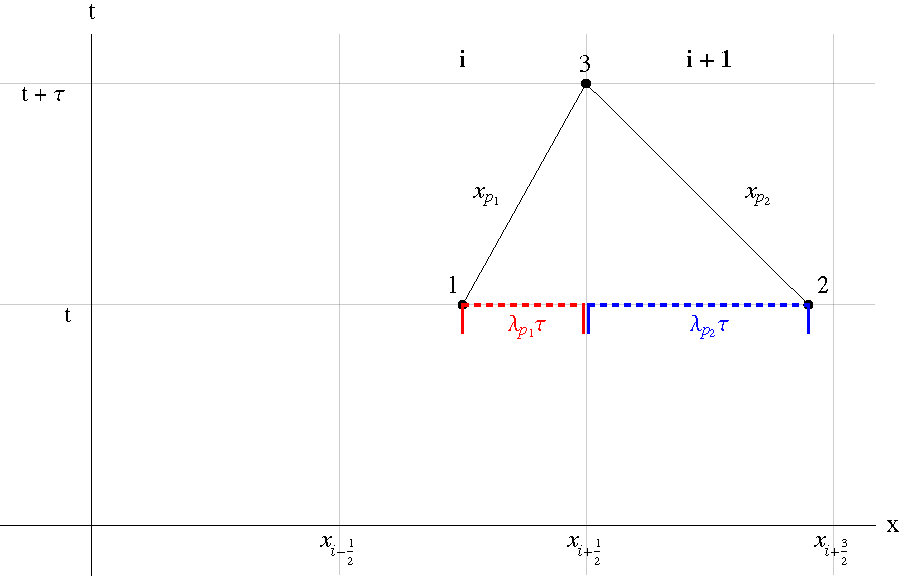
\includegraphics[width=0.7\textwidth]{visualization.pdf}
        \caption{Снос значений по характеристикам на границах разностных ячеек}
        \label{fig:visualization}
    \end{figure}

    \vskip 3cm

    \begin{figure}[h]
        \centering
        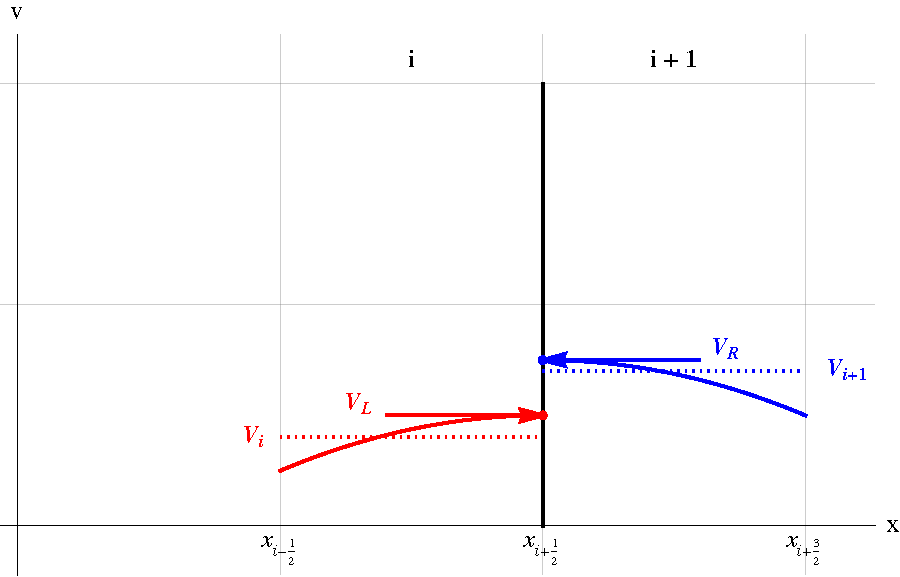
\includegraphics[width=0.74\textwidth]{approximation.pdf}
        \caption{Аппроксимация $\bold v$ в смежных ячейках}
        \label{fig:approx}
    \end{figure}

    \newpage

    \[
        \bold v_i = \dfrac{1}{\Delta x} \int \limits_{x - \half}^{x + \half} \bold v(x) dx.
    \]

    В методе PPM значения $ \bold v_L = \bold v_R $, то есть решения сшиваются, так как используется интерполяционная процедура четвертого порядка. В нашем случае необходимо решать задачу о распаде разрыва между этими состояниями. Для ее решения можно использовать, например, метод Роу:
    \begin{equation}
        \label{row}
        \bold v_{i + \half} = \dfrac{\bold v_L + \bold v_R}{2} + \dhalf \sum_{\lambda_{*p} > 0} \alpha^{*p} \bold r^p (\bold v^*) - \dhalf \sum_{\lambda_{*p} < 0} \alpha^{*p} \bold r^p (\bold v^*),
    \end{equation}
    \noindent где граничные значения $ \bold v_L, \bold v_R $ вычисляются в соответствии с выбранным базисом в ячейках $ i, i + 1 $. Значения правых собственных векторов $ r^p $ вычисляются по состоянию $\bold v^* \colon$
    \[
        \rho^* = \sqrt{\rho^L \rho^R}, \quad \xi^* = \dfrac{\sqrt{\rho^L} \xi^L + \sqrt{\rho^R} \xi^R}{\sqrt{\rho^L} + \sqrt{\rho^R}}, \quad \xi = u,\,\, \dfrac{e + P}{\rho}.
    \]

    Что касается решения системы уравнений газовой динамики в двумерном случае, можно расщеплять ее по пространственным переменным и решать две системы одномерных уравнений вдоль каждой оси координат. Однако при этом необходимо учесть дополнительное изменение величин в граничных точках за счет соответствующих потоков.

    \begin{figure}[h]
        \centering
        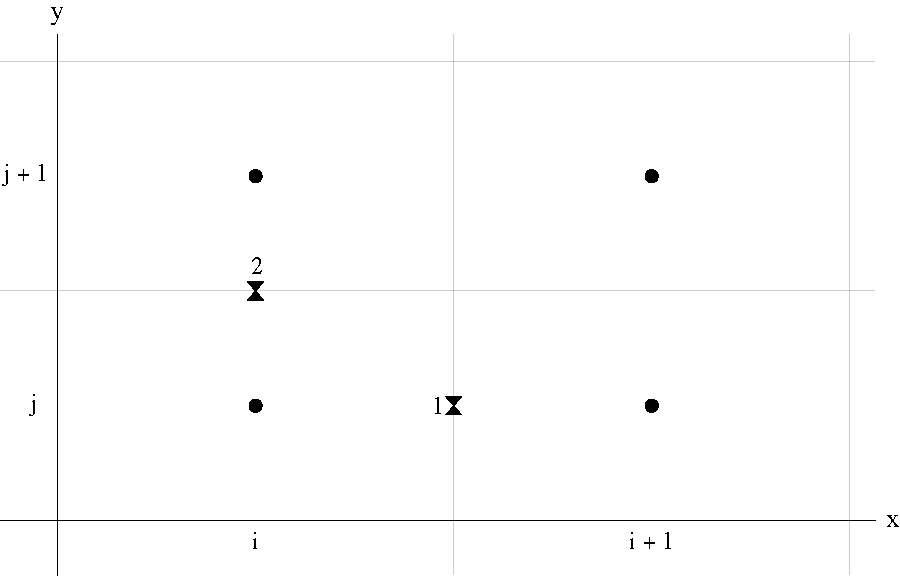
\includegraphics[width=0.6\textwidth]{difference2d.pdf}
        \caption{Двухмерная разностная схема}
        \label{fig:difference2d}
    \end{figure}

    \pagebreak

    Рассмотрим дополнительные изменения величин (\picref{fig:difference2d}). Например, при переходе из ячейки $(i, j)$ в ячейку $(i+1, j)$, что соответствует точке $1$. Изменение величин за счет потока вдоль $Oy$ при переходе к следующему временному слою можно рассматривать как источник и решить систему (\refeq{system:2d}) в направлении $x$, учитывая это слагаемое:
    \[
        \dpartial{\alpha^P}{t} + \lambda^P \dpartial{\alpha^P}{x} = D^p, \quad D^p = -l_x^p A_y^p \dpartial{\bold v^p}{y}.
    \]

    Значения компонент $ \l_x^p, A_y^p $ вычисляются по тому же состоянию, по которому фиксируется базис собственных векторов в ячейке: 
    \begin{itemize}
        \item $(i, j)$ –- для волн, распространяющихся вдоль характеристик с положительными собственными значениями;
        \item $(i, j + 1)$ -- для волн, распространяющихся вдоль характеристик с отрицательными собственными значениями.
    \end{itemize}

    Отметим, что частные производные $\dpartial{\bold v^p}{x}, \dpartial{\bold v^p}{y}$ заменяются разностными аналогами: 
    \[
        \dpartial{\bold v^p}{x} = \dfrac{\bold v_{i+1, j}^p - \bold v_{i, j}^p}{\Delta x}, \quad \dpartial{\bold v^p}{y} = \dfrac{\bold v_{i, j + 1}^p - \bold v_{i, j}^p}{\Delta y}.  
    \]

    Коэффициенты $\alpha^p$ в случае двумерной системы выглядит следующим образом:
    \begin{equation}
        \label{shift:2d}
        \alpha^p(x_{i + \half}, t + \tau) = \alpha^p(x_{i + \half} - \lambda^p \tau, t) + D^p \tau
    \end{equation}

    Левые и правые состояния $\bold v_L, \bold v_R$ в точке $1$, а также граничное состояние $ \bold v_{i + \half, j} $ вычисляются так же, как и в одномерном случае.

    Состояние в точке 2 рассчитывается аналогично, но за счет потока вдоль оси $x$.

    \subsection{Потоки на границах разностных ячеек}

    На состояние в точке, из которой происходит снос по характеристикам на предыдущий временной слой, влияет только интервал от точки пересечения характеристики с кусочной параболой на предыдущем слое до самой точки, т.е. либо $ [x_{i + \half} - \lambda_{\text{pos}} \tau,\, x_{i + \half}] $, либо $[x_{i + \half},\, x_{i + \half} - \lambda_{\text{neg}} \tau] $, обе эти ситуации изображены на \picref{fig:influence}. 

    \pagebreak

    \begin{figure}[h]
        \centering
        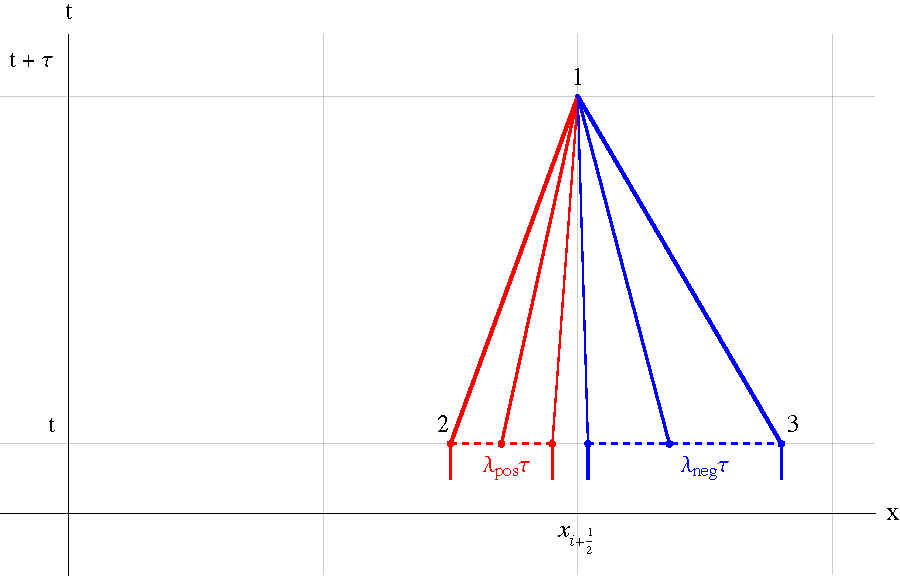
\includegraphics[width=0.8\textwidth]{influence.pdf}
        \caption{Набор характеристик внутри разностной ячейки}
        \label{fig:influence}
    \end{figure}

    Для получение второго порядка аппроксимации по времени нужно усреднить амплитуды $ \alpha^p(x,t) $, отвечающей каждой характеристике, по своей зоне влияния. Пусть внутри ячейки $i$ распространяется вдоль волны с $\lambda^p > 0$, тогда ее усредненная амплитуда будет вычисляться по формуле:
    \[
        \overline{\alpha}^p_{i + \half} = \dfrac{1}{\lambda^p \tau} \int \limits_{x_{i + \half} - \lambda^p \tau}^{x_{i + \half}} \alpha^p (x) dx, \quad \lambda^p > 0,
    \]
    \noindent и если учесть, что 
    \[
      \bold v_{i + \half}^{L, p} = \alpha^p (x) r^p \Rightarrow \alpha^p (x) = l^p \bold v_{i + \half}^{L, p},
    \]
    \noindent получаем
    \[
        \overline{\alpha}^p_{i + \half} = \dfrac{1}{\lambda^p \tau} \int \limits_{x_{i + \half} - \lambda^p \tau}^{x_{i + \half}} l^p \bold v_{i + \half}^{L, p} (x) dx.
    \]

    Базис собственных векторов фиксирован в каждой точке, поэтому его можно вынести из-под знака интеграла, а значит 
    \[
        \overline{\alpha}^p_{i + \half} = l^p \dfrac{1}{\lambda^p \tau} \int \limits_{x_{i + \half} - \lambda^p \tau}^{x_{i + \half}} \bold v_{i + \half}^{L, p} (x) dx = l^p \, \overline{\bold v}_{i + \half}^{L, p},
    \]
    \noindent где $ \overline{\bold v}_{i + \half}^{L, p} $ -- фиксированное состояние, по которому будет выбираться базис собственных векторов. Все характеристики в ячейке $ i $ с отрицательными собственными значениями (в ячейке $i + 1$ -- с положительными собственными значениями) не влияют на состояние в точке $1$. Тогда $\overline{\alpha}^p_{i + \half}$ при $\lambda_p < 0$ ($\lambda_p > 0$) можно либо приравнять к $0$, либо записать через систему:
    \[
        \begin{cases}
            l^p \Bigl(\overline{\bold v}_{i + \half}^{L, 1}\Bigr) \cdot \overline{\bold v}_{i + \half}^{L, p}, & \lambda^p > 0, \\
            l^p \Bigl(\overline{\bold v}_{i + \half}^{L, 1}\Bigr) \cdot \overline{\bold v}_{i + \half}^{L, 1}, & \lambda^p < 0.
        \end{cases}
    \]

    Таким образом, состояние слева от границы $ \bold v_{i + \half} $ получается путем суммирования амплитуд по формуле (\refeq{eq:eigen}), однако удобнее использовать формулу для приращения вектора состояния по базису правых собственных векторов:
    \[
        \overline{\alpha}^p_{i + \half} = \Theta (\lambda^p) l^p \Bigl(\overline{\bold v}_{i + \half}^{L, p}\Bigr) + (1 - \Theta(\lambda^p))l^p \Bigl(\overline{\bold v}_{i + \half}^{L, 1}\Bigr),
    \]
    и если домножить это выражение слева на $r^p$, получим
    \begin{equation}
        \label{value:l}
        \bold v^L_{i + \half} - \overline{\bold v}_{i + \half}^{L, 1} = \sum_{p^+} r^p \Bigl( l^p \Bigl( \overline{\bold v}_{i + \half}^{L, p} - \overline{\bold v}_{i + \half}^{L, 1} \Bigr) \Bigr)
    \end{equation}
        
    Те же рассуждения применимы и для состояния справа от границы $\bold v^R_{i + \half} \colon$
    \begin{equation}
        \label{value:r}
        \overline{\bold v}_{i + \half}^{R, 1} - \bold v^R_{i + \half} = \sum_{p^-} r^p \Bigl( l^p \Bigl( \overline{\bold v}_{i + \half}^{R, p} - \overline{\bold v}_{i + \half}^{R, 1} \Bigr) \Bigr)
    \end{equation}

    Формулы (\refeq{value:l}, \refeq{value:r}) показывают, что приращение каждой физической переменной в окрестности границы складывается из соответствующих приращений этих величин при пересечении каждой характеристики слева направо от одного состояния к другому.

    В конце концов, определим поток $\bold F^{n + \half}_{i + \half}$ на правой границе, воспользовавшись методом Роу. Необходимо обратно перейти к консервативным переменным $\bold u$, затем вычислить $\bold F^L =\bold F(\bold u^L_{i + \half}),\, \bold F^R = \bold F(\bold u^R_{i + \half})$ -- потоки с обеих сторон, после чего воспользоваться формулой:
    \[
        \bold F^{n + \half}_{i + \half} = \dfrac{\bold F_L + \bold F_R}{2} - \dhalf \sum_p |\lambda^p (\bold v^*)| \Delta \alpha^p_{i + \half} r_{\bold u}^p (\bold u^*), \quad \Delta \alpha^p_{i + \half} = l^p (\bold v^*) \Bigl( \bold v^R_{i + \half} - \bold v^L_{i + \half} \Bigr),
    \]

    \pagebreak 

    \noindent где $r_{\bold u}^p$ -- правый собственный вектор консервативной системы газовой динамики.

    \section{Тестирование}

    \begin{center}
        *** В ПРОЦЕССЕ ****
    \end{center}
    \begin{center}
        *** В ПРОЦЕССЕ ****
    \end{center}
    \begin{center}
        *** В ПРОЦЕССЕ ****
    \end{center}
    \begin{center}
        *** В ПРОЦЕССЕ ****
    \end{center}

    \section-{Заключение}

    Рассмотрен кусочно-параболический метод на локальном шаблоне. Выбор в пользу использования решений с предыдущего временного слоя, вместо интерполяционной процедуры, оказался удачным, так как обеспечивает более точное решение и уменьшенную диссипацию. Метод PPML протестирован на ряде примеров, рассмотренных с различными шагами, числами Куранта и профилями. Точность оценивалась на основе норм разности между точным и численным решениям в пространствах $ C,\, L_1,\, L_2 $. В пространствах $L_1, \, L_2$ PPML оказался точнее во всех случаях. Однако в пространстве $C$ результат нельзя интерпретировать однозначно. Но как уже отмечалось, актуальной является сходимость нормы ошибки в $L_2$.

    \newpage

    \begin{thebibliography}{9}
  
        \bibitem{Corella} Corella P., Woodward P. The piecewise parabolic method for gas-dynamical simulations // J. Comput. Phys. $1984$. -- P. $174-201$.
  
        \bibitem{Article} М.\,В.\,Попов, С.\,Д.\,Устюгов. Кусочно-параболический метод на локальном шаблоне для задач газовой динамики // Ж. вычисл. матем. и матем. физ., $2007$. -- C. $2056-2060$.
  
        \bibitem{Galanin} Галанин М. П., Савенков Е. Б. Методы численного анализа математических моделей. -- М. : Изд-во МГТУ им. Н. Э. Баумана, 2018. -- 591~с.

        \bibitem{Samarsky} А.\,А.\,Самарский, Ю.\,П.\,Попов. Разностные методы решения задач газовой динамики. -- M.: Наука. Гл. ред. физ. мат. лит., $1992$. -- $424$ с.

        \bibitem{Kulikovsky} А.\,Г.\,Куликовский, Н.\,В.\,Погорелов, А.\,Ю.\,Семенов. Математические вопросы численного решения гиперболических систем уравнений. -- М.: ФИЗМАТЛИТ, $2001$. -- $608$ с.
  
    \end{thebibliography}

\end{document}